\documentclass[11pt]{article}
\usepackage{jaetakkim}
\usepackage{clrscode3e}


\title{Persistency Analysis}
\author{}
\date{\today}

\begin{document}

\maketitle

\section{Introduction}
An instruction \texttt{write A} persists at program point $v'$ as long as every path from the write to $v'$ has a \texttt{clwb A} followed by \texttt{sfence}.
\[\texttt{write A} \cdots \texttt{clwb A} \cdots \texttt{sfence} \cdots v'\]
with no other writes to the same location between the write and $v'$.

Likewise, \texttt{write A} persists before \texttt{write B} if $v'=\texttt{write B}$ and \texttt{write A} persists at $v'$.
\[\texttt{write A} \cdots \texttt{clwb A} \cdots \texttt{sfence} \cdots \texttt{write B}\]
Note that this only checks for ordering between particular writes, not general writes at these memory locations. That is, there could be another \texttt{write B} instruction that occurs before $v'$ and \texttt{sfence}, so that $A$ doesn't necessarily persist before the other write to $B$.

\section{Problem Formulation}
\subsection{Direction of approximation}
If we formulate the problem such that the existence of a $L$-path from a write to $v'$ gives that the write persists at $v'$, then that only shows that some possible program execution exists where the persist is guaranteed. That is, we let $L$ represent paths that correctly give the right sequence of persist instructions. If there are other paths from the write to $v'$ that isn't in $L$, then other program executions may not have this persistence. Thus, we must have that \textit{every} path is in $L$ to get the guarantee of persistence across all paths taken.

The other direction is to let $L$ represent sequences of instructions that doesn't guarantee the persistence of the write. Then if a $L$-path exists from a write to $v'$ shows that there is some program execution where the persist is \textit{not} guaranteed at $v'$. The false positives here are cases where a $L$-path exists but is never taken in execution, and the only paths that actually execute are paths that \textit{do} guarantee persistence. I think this formulation makes more sense.


\subsection{Formulation}
Given program points $v,v'$ in the CFG, where the instruction at $v$ is a write instruction to location $A$, the write potentially doesn't persist at $v'$ (right before the statement runs) if either there doesn't exist a path from $v$ to $v'$ or if there exists a $L$-path from $v$ to $v'$.

These are the potential ways that a write to $A$ could not persist at $v'$:
\begin{enumerate}
    \item \texttt{clwb A} doesn't exist in the path.
    
    \item \texttt{sfence} doesn't exist after \texttt{clwb A}.
    
    \item (*)There is another write to the same memory location.
\end{enumerate}
(*)We don't need the last way if know that $v$ is the last write to $A$ before $v'$.

\subsubsection{Instructions}
In the intraprocedural setting, with the usual control flow instructions, we also have
\[\textnormal{Stmt} \rightarrow \cdots \;\vert\; \texttt{write x} \;\vert\; \texttt{clwb x} \;\vert\; \texttt{sfence}\]
where $x$ is a location in memory and \texttt{write x} is just some instruction of the form $x := e$ for some expression $e$.

\subsubsection{Language}
In the CFG, we add to the outgoing edges for every statement of the form \texttt{clwb x} the label $\textnormal{wb}_{x}$. To \texttt{sfence}, we add the label $\textnormal{sf}$. Every other edge has empty label $\varepsilon$. We let the alphabet of the language $\Sigma = \{\textnormal{wb}_x\}_{x\in X} \cup \{\textnormal{sf}, \varepsilon\}$, where $X$ is the set of all memory locations. If we are not assuming that the given program point for the write is the last write to the location before $v'$, then we need to add $w_A$ to the alphabet to signify writes. Further, if we wanted one single $L$, rather than a specific $L$ for every two program points, we need to add write edge labels.

The following are the regular expressions that correspond to the potential ways that a write to $A$ does not persist at $v'$:
\begin{enumerate}
    \item $\left(\Sigma - \{\textnormal{wb}_A\}\right)^*$
    
    \item $\Sigma^*\, \textnormal{wb}_A\, (\Sigma-\{\textnormal{sf}\})^*$
    
    \item $\Sigma^*\, w_A\, \Sigma^*$ % Actually idk if we should add edge labels for write instructions. Maybe that requirement isn't needed.
\end{enumerate}
% We're also ignoring incorrect or warning-provoking programs such as a bunch of write backs without the initial writes.

The reachability language $L$ is then either just the first two regular expressions or all three of them:

\[L=\left(\Sigma - \{\textnormal{wb}_A\}\right)^* \;\vert\; \Sigma^*\, \textnormal{wb}_A\, (\Sigma-\{\textnormal{sf}\})^* \quad \textnormal{or} \quad \left(\Sigma - \{\textnormal{wb}_A\}\right)^* \;\vert\; \Sigma^*\, \textnormal{wb}_A\, (\Sigma-\{\textnormal{sf}\})^* \;\vert\; \Sigma^*\, w_A\, \Sigma^*\]

\section{Additions from Px86}
The operational semantics given in Raad et al.\ (POPL '20) paper gives additional persistency-related instructions present in the x86 ISA. There are the two RMW instructions \texttt{FAA}$(x,v)$ and \texttt{CAS}$(x,v,v'')$, another fence \texttt{mfence}, and the two other persist operations $\texttt{flush}_{\textnormal{opt}}$ and \texttt{flush}. Since $\texttt{flush}_{\textnormal{opt}}$ has equivalent specifications to \texttt{clwb}, we will only consider the addition of \texttt{flush}. Note that although \texttt{flush} simplifies persistency guarantees, it is a slower operation than \texttt{flush}$_{\textnormal{opt}}$, which is itself slower than \texttt{clwb}.

The two additional ways that we get a persistence guarantee that one write occurs before another write is if we have \texttt{flush} between the two writes (without the need for fences), or the second write is a RMW instruction (then no fences are required). For durability or ordering guarantees, the addition of the \texttt{mfence} instruction works the same way as \texttt{sfence} (the actual difference between them is that \texttt{sfence} allows for reordering with later reads while \texttt{mfence} does not). Thus, we can easily allow for the substitution of \texttt{sfence} for \texttt{mfence}.

\subsection{flush}
Let's first deal with the addition of the \texttt{flush} instruction. Now there are two ways for a write instruction to have a durability or ordering guarantee: 

\begin{enumerate}
    \item $\texttt{write A} \cdots \texttt{clwb A} \cdots \texttt{sfence}/\texttt{mfence} \cdots v'$
    \item $\texttt{write A} \cdots \texttt{flush A} \cdots v'$
\end{enumerate}

A path has to be not of both forms for the persistency guarantees to not hold. So either both \texttt{flush A} and \texttt{clwb A} does not exist in the path or \texttt{flush A} does not exist, \texttt{clwb A} exists, but no fences. That is,

\[L = \left( \Sigma - \left\{ \textnormal{fl}_A, \textnormal{wb}_A \right\} \right)^* \;\vert\; \left( \Sigma - \left\{ \textnormal{fl}_A \right\} \right)^* \textnormal{wb}_A \left( \Sigma - \left\{ \textnormal{fl}_A, \textnormal{sf}, \textnormal{mf} \right\} \right)^*\]

\subsection{RMW instructions}
If we want an ordering guarantee where the second write is a read-modify-write (RMW) instruction, then we do not need a fence after \texttt{clwb} instruction. The reasoning is that x86 guarantees stricter ordering between RMW instructions and other writes. More concretely, the ordering guarantee of Px86$_{\textnormal{sim}}$ specified by the M-RMW operational semantics rule ensures that the buffer be empty before the RMW instruction is added directly onto the persistency buffer. That is, the first write instruction and its persist operation must be debuffered into the persistency buffer before the RMW instruction gets added to the persistency buffer. Then this guarantees that these instructions are executed in this order. Thus, the path from \texttt{write A} to \texttt{write B} where the second write is a RMW instruction does not guarantee ordering only if no persist operation on $A$ exists in the path.

\[
    L = \left( \Sigma - \left\{ \textnormal{fl}_A, \textnormal{wb}_A \right\} \right)^* 
\]

\subsection{Persistency Buffer and Operational Semantics}
If we examine the operational semantics for the persistent memory model as described in the Raad et al.\ paper, we can get a better handle on what is required for persistency ordering between two write instructions. 

Let $x,y \in \textsc{Loc}$ where \textsc{Loc} is the set of all memory locations. Let $v,v'$ be values. Write instructions (both direct stores and RMW's) are of the form $\langle x, v \rangle$ and persist instructions are of the form $\langle \textnormal{per}, x \rangle$. Examining the two operational semantics rules for debuffering from the persistency buffer (PB), we can deduce that the only way a later write $\langle y, v' \rangle$ can be reordered before an earlier write $\langle x,v \rangle$ (assuming $x,y$ are not on the same cache line) is if there exists a persist operation $\langle \textnormal{per}, x \rangle$ between the two writes. Thus, the order in which the instructions are added to PB must be of the form $\langle x, v \rangle, \ldots, \langle \textnormal{per}, x \rangle, \ldots, \langle y,v' \rangle$. 


\section{PMDK}
For checking persistency using the PMDK operations \texttt{TX_BEGIN}, \texttt{TX_END}, and \texttt{TX_ADD}$()$, we can either run the graph reachability from every write instruction between \texttt{TX_BEGIN} to \texttt{TX_END} to the program point at \texttt{TX_END}. If using \texttt{TX_ADD}$()$ function instead of the low-level persist operations, we only need to check that for every write operation, a corresponding \texttt{TX_ADD}$()$ operation exists before the write.


\section{Today}
\subsection{Language}
The language that describes paths \textit{not} in the language for paths. That is, it represents paths that do guarantee persistence.
\begin{align*}
    L^{c} & \to w_{x_1}\, T_1\, b_{x_1}\, T_1\, f_s\, T_1 \;\vert\; \cdots \;\vert\; w_{x_k}\, T_k\, b_{x_k}\, T_k\, f_s\, T_k \\
    T_1 & \to w_{x_2} \;\vert\; \cdots \;\vert\; w_{x_k} \;\vert\; b_{x_1} \;\vert\; \cdots \;\vert\; b_{x_k} \;\vert\; T_1 \, T_1 \;\vert\; f_s \;\vert\; \varepsilon \\
    \vdots & \\
    T_k & \to w_{x_1} \;\vert\; \cdots \;\vert\; w_{x_{k-1}} \;\vert\; b_{x_1} \;\vert\; \cdots \;\vert\; b_{x_k} \;\vert\; T_k \, T_k \;\vert\; f_s \;\vert\; \varepsilon\\
\end{align*}
where there are $k$ unique variables, $w_x$ represents a write to $x$, $b_{x}$ represents a \texttt{clwb} $x$ statement, and $f_s$ represents a \texttt{sfence} statement. The $T_i$ rule represents a string of any length and any terminals except the $w_{x_i}$ terminal.

Or written as a regular expression:
\[L^c = w_{x_1}\, T_1 \, b_{x_1}\, T_1\, f_s\, T_1 \;\vert\; \cdots \;\vert\; w_{x_k}\, T_k\, b_{x_k}\, T_k\, f_s\, T_k \qquad \textnormal{where }T_i = \left( \Sigma - \left\{ w_{x_i} \right\} \right)^*\]


If we consider only paths that start with a write (because it doesn't make sense to ask about persistence of a non-write), then these are the ways that a path can represent a non-persistence:
\begin{enumerate}
    \item Doesn't start with a write:
    \[
        \left( \Sigma - \left\{ w_{x_1}, \ldots, w_{x_k} \right\} \right) \Sigma^*
    \]

    \item Write to the same variable appears again:
    \[
        w_{x_1} \Sigma^* w_{x_1} \Sigma^* \;\vert\; \cdots \;\vert\; w_{x_k} \Sigma^* w_{x_k} \Sigma^*
    \]
    \item There's no \texttt{clwb} after the write:
    \[
        w_{x_1} \left( \Sigma - \left\{ b_{x_1} \right\} \right)^* \;\vert\; \cdots \;\vert\; w_{x_k} \left( \Sigma - \left\{ b_{x_k} \right\} \right)^*
    \]
    \item There's no \texttt{sfence} after the \texttt{clwb}:
    \[
        w_{x_1} \left( \Sigma - \left\{ w_{x_1} \right\} \right)^* b_{x_1} \left( \Sigma - \left\{ f_s \right\} \right)^* \;\vert\; \cdots \;\vert\; w_{x_1} \left( \Sigma - \left\{ w_{x_k} \right\} \right)^* b_{x_k} \left( \Sigma - \left\{ f_s \right\} \right)^*
    \]
\end{enumerate}

The a path is in the language $L$ if it's in any of the languages specified by the regular expressions above.

\newpage
\subsection{Example}
\begin{codebox}
  \Procname{\proc{Program 1}}
  \li $x \gets 6$
  \li \texttt{clwb} $x$
  \li \texttt{sfence}
  \li \While $x > 0$:
  \Do
    \li \If $x>5$:
    \li \Then $x \gets 0$
        \li \texttt{clwb} $x$
    \li \Else
    \li $x \gets x - 1$
        \End
    \li \texttt{sfence}
  \End
  \li \texttt{output} $x$
\end{codebox}

\begin{figure}[h]
    \centering
    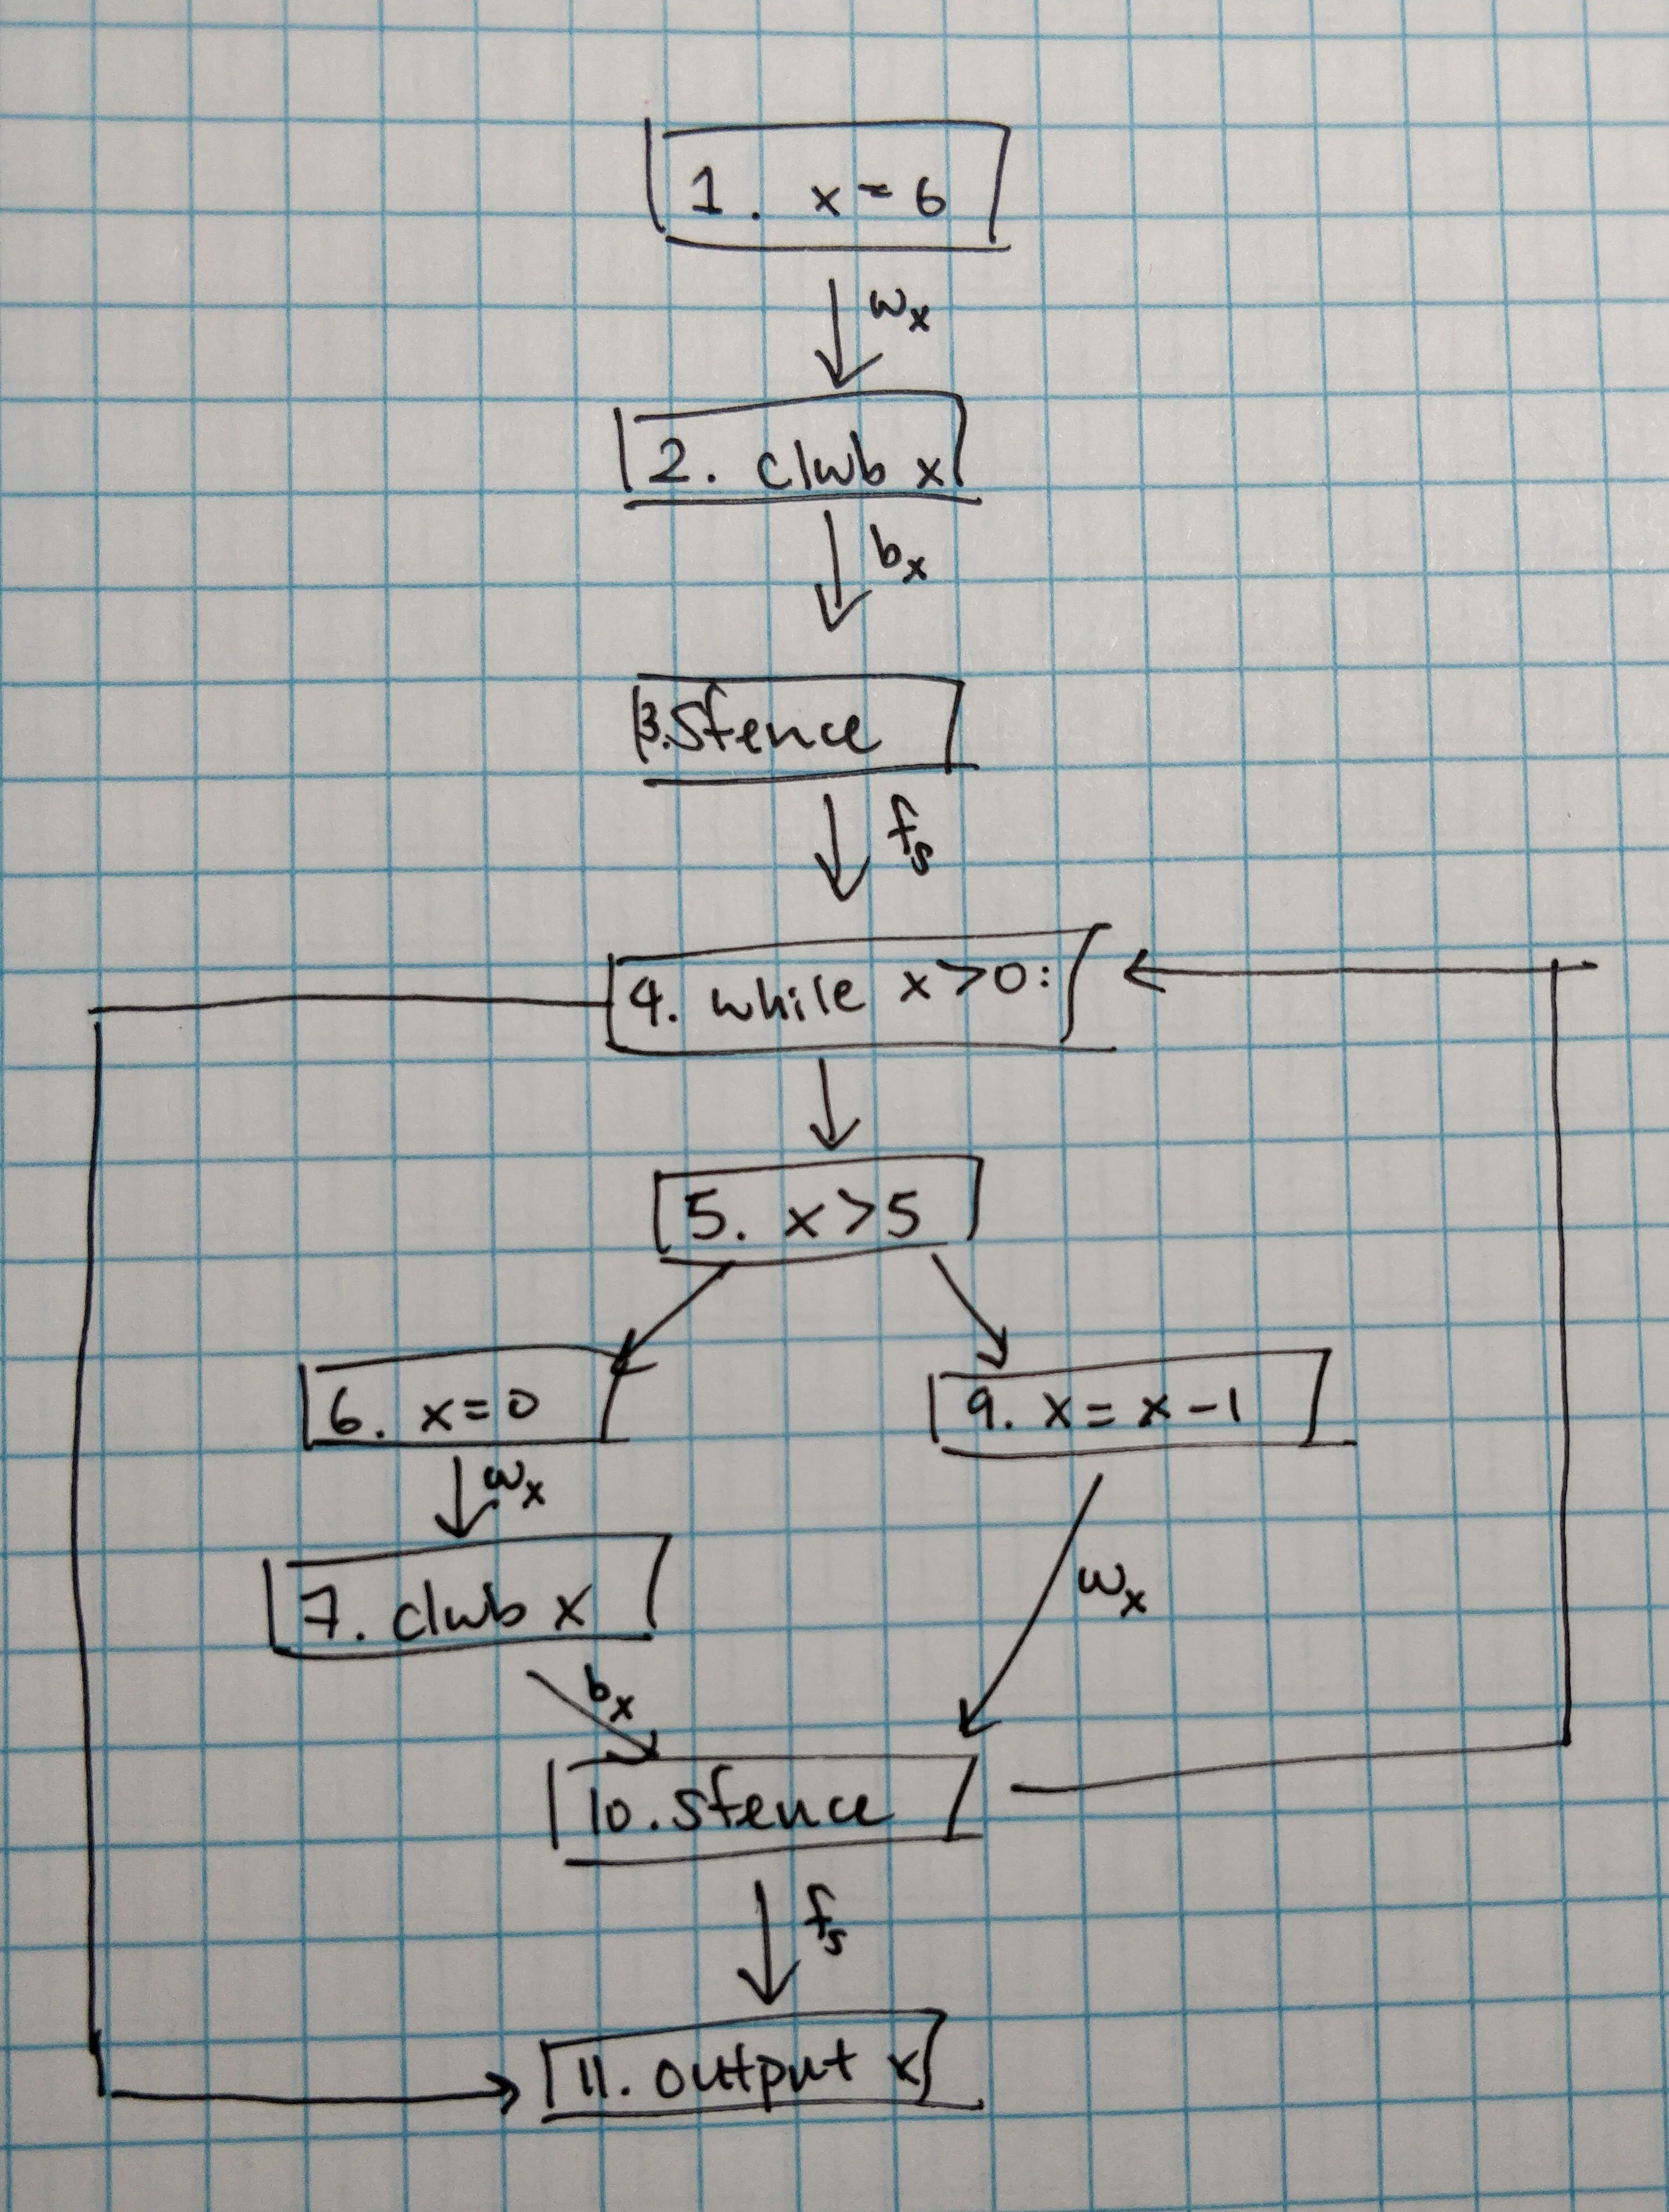
\includegraphics[scale=0.08]{ex-cfg}
\end{figure}
There is a path that is potentially non-persistent from every write to the last line. The actual path that this program will take upon execution will have the path string $w_x b_x f_s w_x f_s \in L$, so it isn't persistent, and neither is it from the second write to the last line.

\newpage
\subsection{PMDK: libpmemobj}
(From \textit{Programming Persistent Memory by Scargall} book)

3 API's to persist data to memory:
\begin{enumerate}
    \item Atomic operations -- simplest and fastest but limited to allocating and initializing wholly new blocks.
    \item Reserve/publish -- can be almost as fast as atomic but can't read data you just wrote.
    \item Transactional -- most flexible but slowest.
\end{enumerate}

\noindent Transactional API:
\begin{figure}[h]
    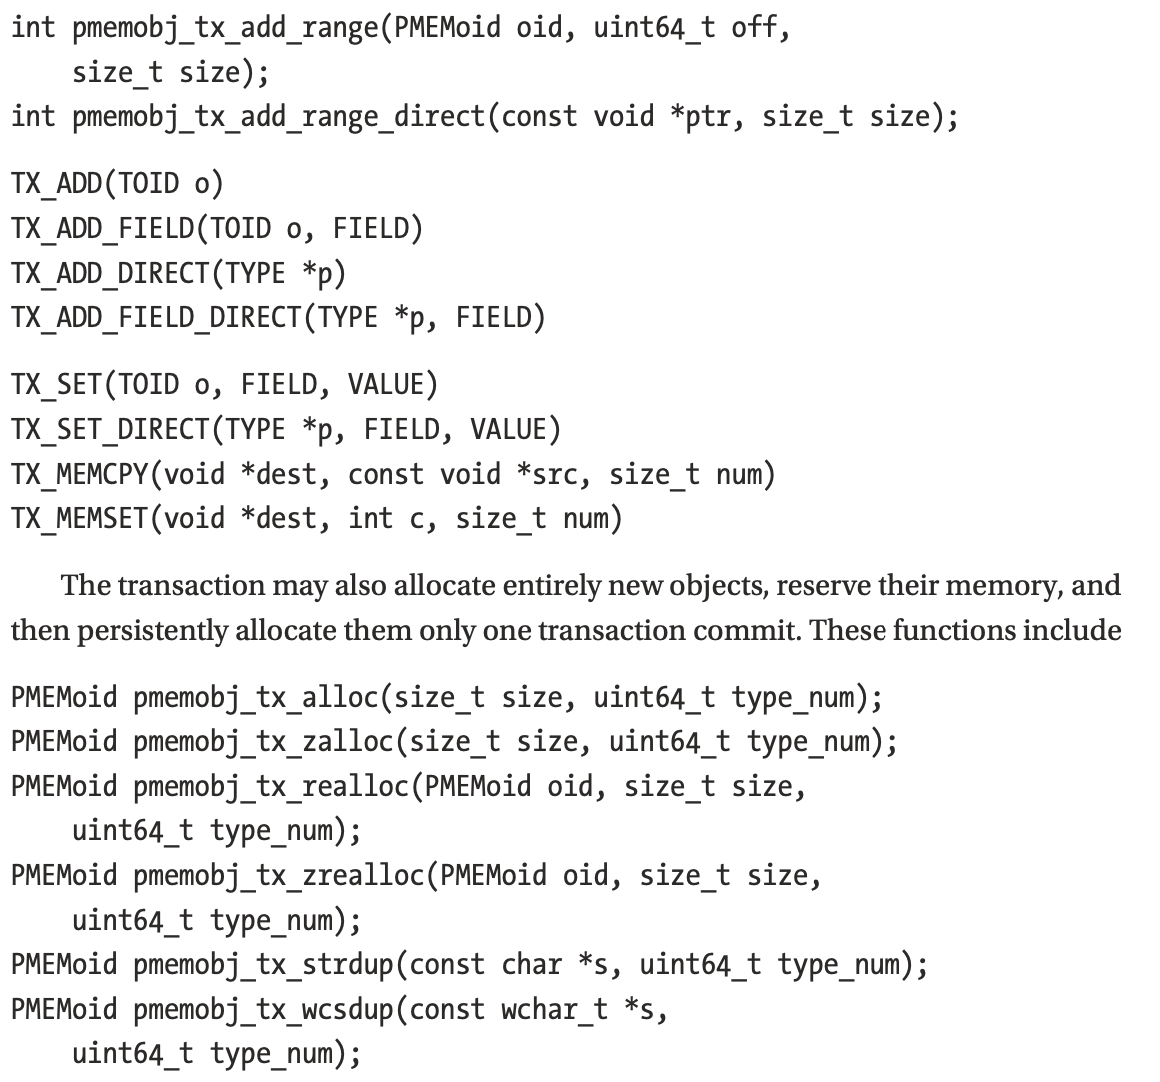
\includegraphics[scale=0.6]{libpmemobj-tx}
\end{figure}


\newpage
\section{Enforcing Persist Ordering}
\subsection{PMTest Liu et al.}
Here are the relevant PMTest operations copied from the paper:
\begin{itemize}
    \item \texttt{global_timestamp} \textbf{(global status):} A global epoch counter that is incremented on every \texttt{sfence} encountered in the trace.
    \item \texttt{persist_interval} \textbf{(local status):} The interval in which certain memory location(s) may persist.
    \item \texttt{flush_interval} \textbf{(local status):} The interval in which certain memory location(s) may be explicitly written back to PM.
    \item \texttt{write(addr,size)} modifies an address range of [addr, addr+size) in the shadow memory. It first clears existing \texttt{persist_intervals} and \texttt{flush_intervals} within the address range and sets the \texttt{persist_intervals} as (\texttt{global_timestamp}, \(\infty\)). That is, this write may persist at any time moving forward.
    \item \texttt{clwb(addr,size)} writes back an address range of [adddr,addr+size) and the \texttt{flush_interval} is set as (\texttt{global_timestamp},\(\infty\)). That is, a writeback for these addresses has been issued and it may happen at any time moving forward. If there is an existing \texttt{flush_interval}, PMTest raises a \texttt{WARNING}.
    \item \texttt{sfence} enforces the ordering of prior \texttt{write} and \texttt{clwb} operations. First, it increments the \texttt{global_timestamp}. Second, it updates the \texttt{flush_interval} of prior \texttt{clwb}s so that the intervals end at the current \texttt{global_timestamp}, i.e, the writeback is complete. Third, it updates the \texttt{persist_interval} of prior \texttt{clwb}s so that the intervals end at the current \texttt{global_timestamp}, i.e, the write persisted.
    \item \texttt{isOrderedBefore(addrA,sizeA,addrB,sizeB)} checks whether \textit{all} writes to [addrA,addrA+sizeA) can persist before any write to [addrB,addrB+sizeB) by checking if any of the \texttt{persist_intervals} in [addrB,addrB+sizeB) overlap with any of those in [addrA,addrA+sizeA).
\end{itemize}

The checking rule \texttt{isOrderedBefore}\((A,B)\) checks if the persist intervals of \(A\) and \(B\) overlap. The start of PI's are only set by a \texttt{write} to the address and it is set to the current \texttt{global_timestamp}. The end of a PI is only changed by an \texttt{sfence} operation where it is set to \texttt{global_timestamp} if there was a previous \texttt{clwb} operation to the same address. Because \texttt{global_timestamp} is incremented only by an \texttt{sfence} operation and is never decremented, this implies that there \textit{\textbf{must}} be a \texttt{sfence} before the last write to \(B\) (the write that is being checked for persist ordering).

Suppose that there isn't a \texttt{sfence} between \texttt{write}\((A)\) and \texttt{write}\((B)\) but that an \texttt{sfence} occurs after both writes. Let \(\left( a_1, a_2 \right)\) be the PI for \(A\) and let \((b_1, b_2)\) be the PI for \(B\). The intervals overlap if \(b_1 < a_2\). At this \texttt{sfence} call, the first thing that occurs is that \texttt{global_timestamp} is incremented. Then \(a_2\) is set to this new \texttt{global_timestamp}, assuming that a \texttt{clwb}\((A)\) exists before the \texttt{sfence} (if this wasn't the case, \(a_2\) would never be changed from \(\infty\) so \(b_1 < a_2\) always). But note that this \(a_2\) must be strictly greater than \(b_1\) because \(b_1\) was set by some previous \texttt{global_timestamp} and the \texttt{sfence} operation just incremented \texttt{global_timestamp}. So unless \(b_1\) is over-written by another \texttt{write}\((B)\), \(b_1 < a_2\) and the intervals overlap.

% Furthermore, \texttt{sfence} only updates the end of a PI for addresses that have a \texttt{clwb} to them, so there must also be a \texttt{clwb}\((A)\) before the previously mentioned \texttt{sfence}.

\begin{note}
So it might just be that everything is simple as long as you don't consider rewrites. Well actually, it might be that there are multiple PI inside a single range of addresses. I'm thinking of arrays. There's also performance ``bugs'' that PMTest checks for.
\end{note}

Maybe also think about interprocedural and weird functions and loops and threads and other things like that that could mess things up. Also, note that PMTest only works for a particular execution whereas static program analysis will probably be flow-insensitive. How does the interaction of multiple \texttt{clwb} within the same address range interact with a single overall write? What's the point of maintaining \texttt{flush_interval}?


\subsection{Operational Semantics}

\end{document}
